\subsection{Entity-Relationship Schema}

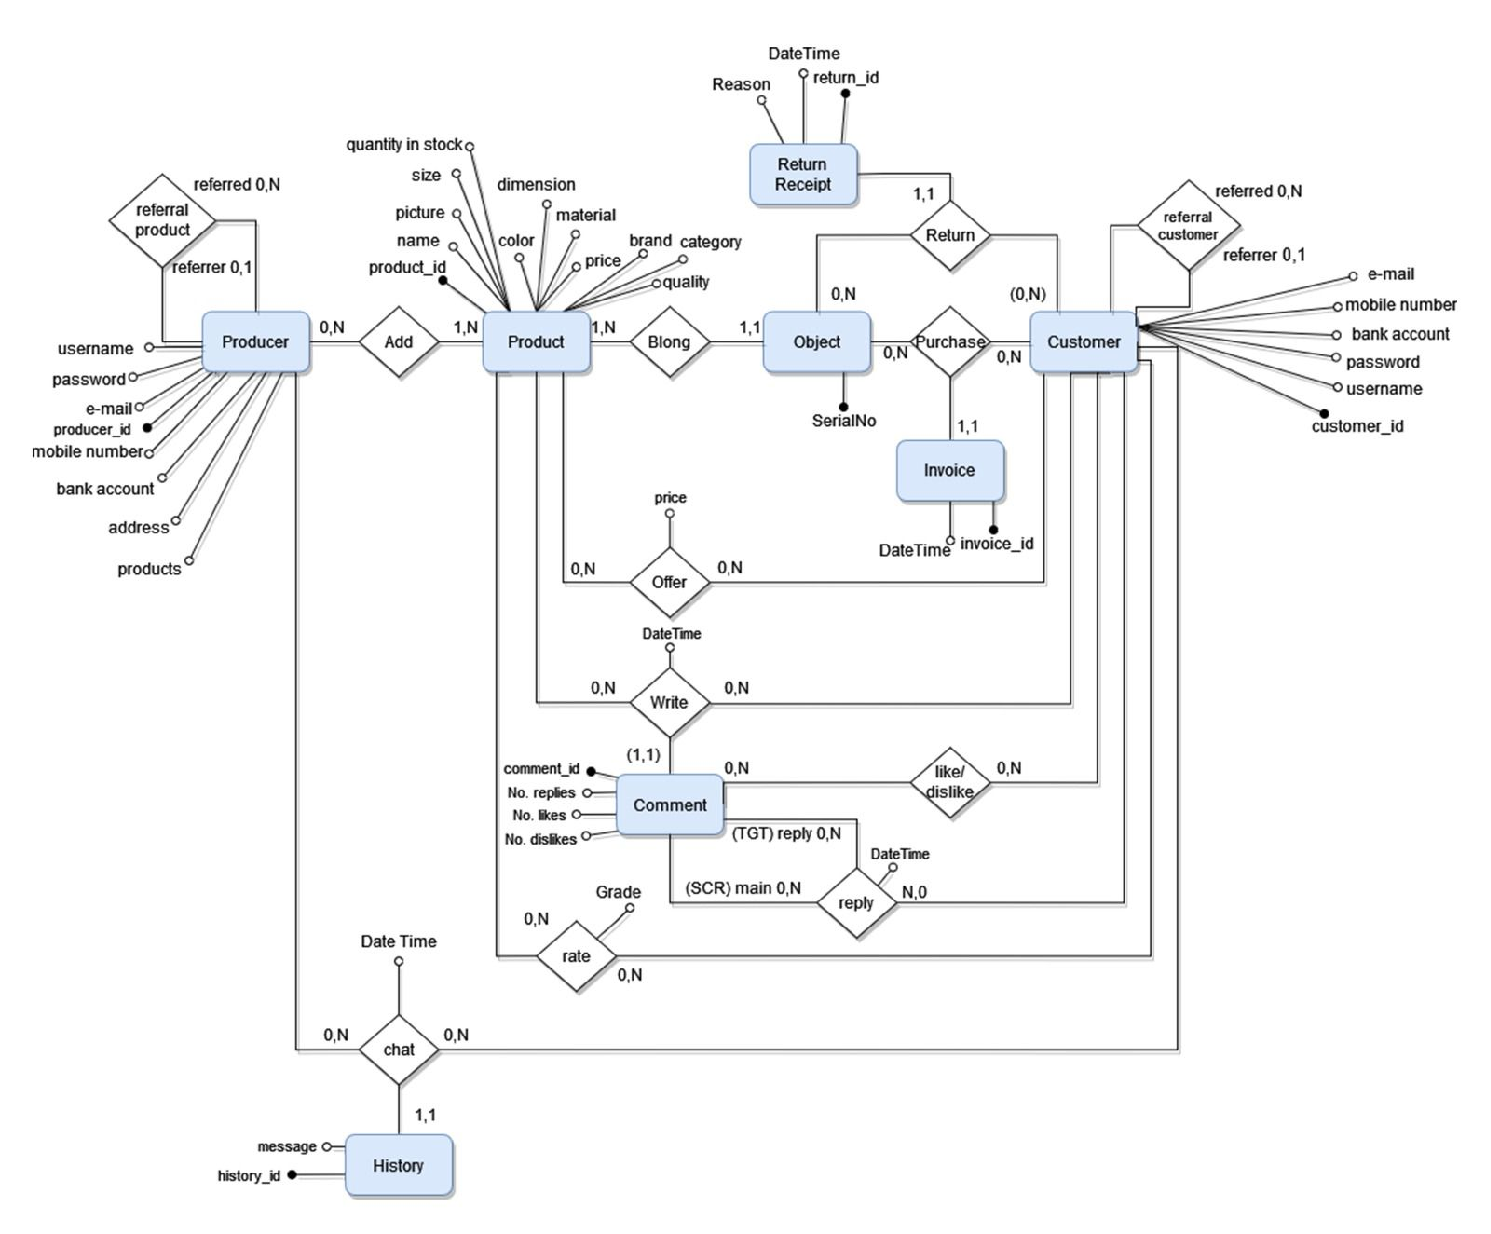
\includegraphics[scale=0.7]{wab-homework1/logos/ERSchema.pdf}

%Describe here your ER schema

\noindent The entity-relationship schema contains 8 main entities:
\begin{itemize}
    \item Customer: Each customer has unique details that distinguish them from other customers. Customers can order or purchase products, leave comments expressing their opinions about products, and engage in chats with producers.
    \item Object: Objects are a subset of products, meaning that there can be different versions of each product that customers can purchase, known as objects. Objects are distinguished by serial numbers.
    \item Product: Producers supply the products, and customers can suggest a price for the products, allowing for bargaining. Producers can accept or reject the price or leave a comment related to the product. Customers can also rate and leave comments for products.
    \item Producer: Producers are responsible for adding products to the platform, and customers can communicate with them directly.
    \item Return receipt: If a customer returns a product, a receipt titled "return receipt" is issued, containing details related to the returned product.
    \item Invoice: When a customer purchases an object, a receipt is issued containing the details of the product and the purchase.
    \item Comment: Customers can leave comments for products, which can be liked or disliked, with the ability to reply to comments. The details of these comments are saved.
    \item History: This entity stores the history of direct communication between each customer and producer to avoid duplicate data in case of re-connection.
 \end{itemize}

